\documentclass[11pt]{article}
\usepackage{geometry}
\geometry{a4paper, bottom=30mm, top=30mm, left=15mm, right=15mm}
\usepackage{pdfpages}
\usepackage{fancyhdr}
\pagestyle{fancy}
\setlength{\parindent}{0cm}
\setlength{\headheight}{14pt}
\usepackage{tocloft}
\usepackage{parskip}
\usepackage[export]{adjustbox}
\usepackage{float}
\usepackage{subfig}
\usepackage{graphicx}
\graphicspath{{../figures}}
\usepackage{amsmath,blkarray,booktabs,bigstrut, amssymb}
\usepackage{pythonhighlight}
\usepackage{outlines}
\usepackage{soul}
\usepackage[hidelinks]{hyperref}
\usepackage[backend=biber, style=ieee]{biblatex}
\addbibresource{references.bib}
% \bibliographystyle{ieee} % or another style like IEEE, APA, etc.
% \nocite{*}
\usepackage{url}
\setcounter{biburllcpenalty}{7000}
\setcounter{biburlucpenalty}{8000}
\widowpenalty10000
\clubpenalty10000
\setcounter{secnumdepth}{3}
\usepackage[newfloat]{minted}
\usepackage{caption}
\newenvironment{code}{\captionsetup{type=listing}}{}
\SetupFloatingEnvironment{listing}{name=Code Listing}


\begin{document}

\newgeometry{top=20mm}
\begin{titlepage}
    \begin{center}
      \begin{figure}
        
\includegraphics[right]{logo.png}
      \end{figure}
      \vspace*{1cm}
      \textsc{\large ENEL373: Digital Electronics and Devices}\\[0.5cm]
      \textsc{\Large University of Canterbury}\\[3.5cm]
      \linespread{1}
      {\Huge\bfseries This is an Awesome Title \\[0.3cm] for Our First Report} \\
      \vspace*{2cm}
      {\Huge Philip Brand \textit{\Large(15776928)}\\\par}
      {\Huge Michael Brown \textit{\Large(48571923)}\\\par}
      {\Huge Boston Black \textit{\Large(********)}\\\par}
      % ADD YOUR NAME AND STUDENT ID HERE
      \vspace*{3cm}
      {\LARGE \today}
    \end{center}
  \end{titlepage}
\restoregeometry

\fancyhead{}
\fancyhead[L]{\small{ENEL373 - Reaction Timer Project}}
\fancyhead[R]{\small{\today}}

\pagenumbering{roman}

\renewcommand{\baselinestretch}{1.3}\normalsize
\setlength{\cftbeforesecskip}{0.3em}
\renewcommand{\cftsecleader}{\cftdotfill{\cftdotsep}}
\addcontentsline{toc}{section}{Contents}
\tableofcontents\thispagestyle{fancy}
\renewcommand{\baselinestretch}{1}\normalsize

\newpage
\pagenumbering{arabic}

\section{Introduction}
% Outline (in your own words) the project requirements and what you achieved

Human reaction time is the interval between the a stimulus and the response to that stimulus. There are two main types of reaction time; simple, and choice. Simple reaction involves reacting to a singular stimulus, while choice reaction involves choosing the correct response from multiple stimuli. This project aims to implement a simple reaction time recorder on an FPGA in VHDL.

The reaction stimulus test starts with three LEDs that turn off sequentially, with a random delay between each LED turning off. Once the last LED turns off, the user must press a button, and the delay is displayed in milliseconds on 8 7-segment displays. The FPGA stores the reaction delays from the last three trials, and can display the fastest, slowest, and average reaction times. These values can be reset by the user.

\section{Design Summary}
% Summarise your design.

The FPGA reaction stimulus test depends on four major components, those being the 8-digit counter, the ALU, the reaction countdown, and the output select and override. These components are shown in Figure \ref{project_structure}. Each of these components are enabled and disabled via a finite state machine.

\begin{figure}[H]
  \centering
  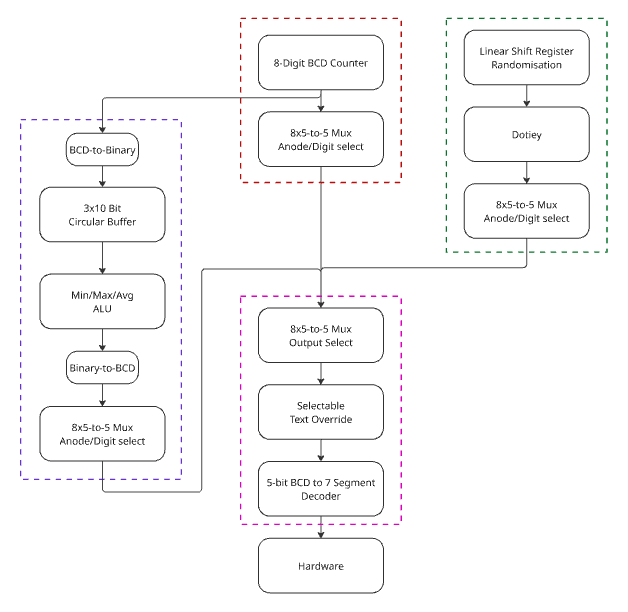
\includegraphics[width=0.7\textwidth]{project_overall_structure.png}
  \caption{Overview of VHDL reaction timer structure}
  \label{project_structure}
\end{figure}

An 8-digit 5-bit-BCD counter is the primary mechanism used to track the reaction time from each stimulus test to the nearest millisecond. Each BCD digit is passed into an 8x5-to-5 mux. The purpose of this mux is to sync the selected output digit with the currently active seven segment display anode, outputting each digit onto its associated display.

All the BCD digits from the 8-digit counter are passed directly to ALU module. This module converts the BCD numbers into a 10-bit binary number, then stores the last three reaction times in a circular buffer. This buffer is read by the ALU which calculates the average, minimum, and maximum of the last three reaction times. These times are converted back into BCD, and another 8x5-to-5 mux is used to select which digit is output.

A linear shift register is used to provide some randomisation for the countdown sequence at the start of every reaction stimulus test. This time randomisation acts as the trigger for the countdown state, Dotiey, and also has an 8x5-to-5 mux for digit selection.

All three 8x5-to-5 muxes from the three components described above are piped into an 8x5-to-5 mux used for output selection. This mux selects which module to take output from depending on what state is active. The mux output is piped into a text override, which overwrites some of the digits with letters based on state. This is finally piped into a 7 segment decoder, which takes a 5-bit BCD digit and converts it to a 8-bit seven segment display light combination which is piped to hardware.



\section{Expanded Design Summary}
% (~2 pages): Describe the methods your group used to implement your FPGA design. Justify your final design. Support your descriptions and justifications with specific, explicit references to your VHDL source code in the appendix. VHDL descriptions could, for example, include an RTL description. 

\subsection{Design Methods}

The primary focus for the reaction timer project project was to develop VHDL code that is easy to maintain and develop. This led to a heavy focus on modular design and code reuse. Since the project was developed as a group, the other focus was for individual components to be developed and tested by individually, and then put together with minimal issues. 

\subsubsection{Diagramming}

The primary program development method used in this project was to draw program or component flow diagrams before VHDL was written. These digrams detailed the communication between between individual modules, and outlined the overall program structure. Figure \ref{project_structure} shows one such digram outlining each major component in the design and how they're grouped into larger modules. 

Clear communication between group members of the expected inputs and outputs from each component played a significant role in keeping the final assembly simple. Examples include the consistent transfer of characters to be displayed 8x5-to-5 muxes to transmit one character at a time unless otherwise required, such as for the ALU.

\hl{Philip - Michael, do you want to cover some of this?}

\subsubsection{Naming and Syntax Conventions}

Another important aspect of the project ensuring high code quality, readability, and maintainability was strict rules around naming and syntax. This included consistent whitespace, indentation, case, and naming style. For example, all signals within the entity was postfixed with an underscore and whether that signal was an input or output. This can be seen in Listing \ref{code:entity_naming_convention} in Appendix A. This ensured when the components were used in the top-level Behavioural architecture with port mapping, it was easy to see which signals were inputs and outputs.

\hl{Add more examples here \dots}

\subsubsection{Component Reuse}

\hl{Philip - I believe you Boston were going to write this?}

\subsubsection{Programming Techniques}

Another method used to implement the FPGA design was pair programming. This had to be done with care, as since the project was done in three-person groups, it would have been easy to leave one person out of the process and result in a lack of their understanding of the code. However, pair programming did help ensure that minimal time was spent debugging, as the observer frequently caught subtleties of VHDL that the programmer missed. Pair programming was used to develop the circular buffer, counters, and FSM.

Since the project the significantly modularised, it was important that individual components could be developed and tested without hindering the development of other components. The method used to achieve this was to use git branching and merging. Individual components were developed on separate branches, tested, and then merged into the main branch. This ensured that the main branch was always stable, and that broken changes could be easily rolled back.

\subsection{Design Justification}

\begin{enumerate}
  \item it did what it was meant to do
  \item it was not coded into an unchangeable spaghetti
  \item it was incredibly modular
\end{enumerate}

\newpage

\section{Module Testing}
% A brief section describing how you tested a significant module. Include at least one testbench and associated waveforms that demonstrate the functionality of a module in the report appendix.

\hl{Philip - I believe this was going to the random number generator and then we can discuss maximal outputs? (to do on Tuesday?)}

\newpage

\section{Design \& Implementation Problems}
% Design and/or Implementation problems (can be a separate section or part of the Conclusion): marks for describing problems encountered, and explaining approach to solving them.
% NB: Marks do not depend on whether problems were solved or not, but on the process used.
% 4 marks


\begin{enumerate}
  \item Steven Weddell
  \item Vivado
  \item Vivado
  \item Vivado
  \item VHDL
  \item Steven Weddell
  \item Steven Weddell
  \item Vivado
  \item Vague Error messages
  \item Decimal point issue
  \item Randomisation delay insufficient
  \item Not case sensitive code
  \item Steven Weddell
  \item Vivado
\end{enumerate}

One issue that arose during the development of the seven segment display module which mapped a BCD input to a combination of segments on a display to represent that BCD number was that the provided mappings did not represent the numbers correctly. The solution approach was to first determine whether the BCD input or mapping was incorrect. This was done by tying the BCD input to the green LEDs on the FPGA. This asserted BCD input was correct. To rectify the incorrect mappings, individual segments on a board were tied to the FPGA user switches. Combinations of switches were tested, and when the segments represented a number, the combination of switches was recorded as a mapping.

However, once all the mappings were implemented, we found that our countdown timer failed to display the dots. Alteration of the countdown timer to display temporary digits instead of dots revealed the countdown to be functional. Stepping through the code by hand revealed that, due to the use of the unfamiliar provided seven segment decoder, a line of code was overlooked that overwrote the decimal place value. Disabling this line of code allowed the countdown timer to show dots.

A significantly unexpected issue that appeared during the testing of the finite state machine was deemed as the "Schrodinger's States" problem. This originated from the FSM running lines of code designed to change states even while they were commented out. In addition, an unwanted state change wouldn't necessarily complete, instead running half of a state's instructions before reverting back to the original state. This was fixed by removing the FSM inputs from the sensitivity list of the FSM process, instead tying it to a 10KHz clock instead. \textcolor{red}{CONFIRM THE CLOCK SPEED}.

There were issues with the simulation software built into the Vivado toolchain. During the design of the BCD-to-Binary numeric convertor, the Vivado simulator would stop the simulation at the beginning of the numeric conversion, but would not give an error message to indicate an issue. However, generating a bitstream and running it on hardware led to no such issues with the BCD-to-Binary module, and the numeric conversion operated as intended.

\newpage

\section{Conclusions}
% Highlight any problems you encountered and how you solved them. Also discuss what you learned and give suggestions on how the project could be improved


\newpage
% There is no need to include a full code listing in your report as your code will be submitted via eng-git. However, reference to a code snippet in an appendix is quite appropriate. Formal citations to books, web articles, open source VHDL code and other sources should be listed in a reference section that uses the IEEE style and format.


\printbibliography

\newpage

\section{Appendix A: Code Listings}


\begin{code}
  \begin{minted}{vhdl}
  
    -- Define module IO
    entity counter_decade is
        Port ( EN_IN : in STD_LOGIC;
               RESET_IN : in STD_LOGIC;
               INCREMENT_IN : in STD_LOGIC;
               COUNT_OUT : out STD_LOGIC_VECTOR (3 downto 0);
               TICK_OUT : out STD_LOGIC);
    end counter_decade;

  \end{minted}
  \captionsetup{belowskip=0pt}
  \captionof{listing}{Entity naming convention example.}
  \label{code:entity_naming_convention}
  \end{code}

\end{document}
